\chapter{Results and Analysis}

\section{Simulated Data}

\subsection{Test Cases}

The test cases looked at were selected to determine the effects of the spacecraft inertia, the spacecrafts orbit and its geometry. In total 18 total cases were simulated, each were simulated at various times of the year with randomized angular velocities.

The geometries used in this analysis were a rectangular prism, a cylinder, and a box-wing. The first two are convex geometries that have differing levels of symmetry, while the box-wing geometry is concave. These geometries can be seen in figure \ref{simulated_geometries}. The orbits examined are Low Earth Orbits (LEO), elliptical Medium Earth Orbits (MEO) and Geostationary (GEO). The final variable is the spacecrafts inertia. In the first case, the pricipal inertial axes are assumed to be aligned with the spacecraft body frame and equal in magnitude. This corresponds to the inertial properties of a uniform sphere. The effect of this is to make the spin axis constant for all time. In the second case, the principal inertial axes are all different and are not aligned with the body frame, causing the spin axis to change over time.

\begin{figure}
	\begin{center}
	\begin{tabular}{cc}
		\includegraphics[width = 50mm]{Long_Rectangle_Image_Axes.png} &
		\includegraphics[width=50mm]{Cylinder_Axes} \\
		Rectangular Prism & Cylinder \\
		\multicolumn{2}{c}{\includegraphics[width=50mm]{Box_Wing_Axes}} \\
		\multicolumn{2}{c}{Box Wing}
	\end{tabular}
	\end{center}
	\caption{Three Simulated Geometries.}
	\label{simulated_geometries}
\end{figure}


%\begin{figure}
%	\begin{center}
%	\begin{tabular}{cc}
%		\includegraphics[width = 50mm]{leo_orbit} &
%		\includegraphics[width=50mm]{meo_orbit} \\
%		Low Earth Orbit (465km x 506km) & Medium Earth Orbit (541km x 21,200km) \\
%		\multicolumn{2}{c}{\includegraphics[width=50mm]{geo_orbit}} \\
%		\multicolumn{2}{c}{Geostationary Orbit (35,786km x 35,786km)}
%	\end{tabular}
%	\end{center}
%	\caption{Three Simulated Orbits.}
%\end{figure}

\begin{figure}
	\begin{center}
		\begin{tabular}{| c | c | c | c | c |}
		\hline Orbit  & Eccentricity & Semimajor Axis & Inclination & Period\\
		\hline LEO & 0.0029656 & 6,864 km & 97.042 & 94.30 min\\
		\hline Eccentric MEO & 0.5989717 & 17,254 km & 31.273 & 375.92 min\\
		\hline GEO & 0.0001267 & 42,164 km & 0.028 & 1436.7 min \\
		\hline
		\end{tabular}
	\end{center}
	\caption{Three Simulated Orbits.}
\end{figure}

		

\subsection{Methodology}

\subsubsection{Simulation Methodology}
First, a LEO, MEO, and GEO orbit were selected. Passes were calculated by brute force sampling a spacecrafts location and checking for necessary conditions. These conditions were obviously that the spacecraft must be above the horizon of the observation site and that the spacecraft be illuminated. Passes lower than 20 degrees elevation were discarded because of their decreased length. Additionally, because this thesis assumed that atmospheric effect were negligible, low elevation passes violate this assumption. Additionally, in preliminary experiments it was noticed that the UKF often failed to converge to a solution when the angle between the observation and sun vector was greater than 90 degrees. This is likely because the probability of any facet to be illuminated and visible drops significantly as the illuminated faces become predominantly on the far side of the object. This increases the indeterminacy of the problem as sometimes as few as only one illuminated surface may be visible. Therefore passes whose observation and sun vectors were separated by more than 90 degrees were also discarded. Passes were also limited to only 5 minutes of data collection as MEO spacecraft passes can be hours long and geostationary passes are perpetual. 

A 5 minute pass provides a significant amount of data, more than enough for the UKF to converge to a result. Additionally, based on the data provided by Lockheed Martin Space, real pass data is rarely collected for more than a few minutes.

Once a pass was identified, the spacecraft was given three initial attitudes and angular velocities between 0.1 and 0.3 radians per second. These were then propagated and used to calculate three different light curves per pass. Before entering the Kalman Filter, Gaussian noise was added to the light curve whose distribution was similar to that of the real data collected. Gaussian noise is standard as the assumption of the Kalman Filter is that the noise processes are distributed in a Gaussian manner \cite{kf_kalman}. The standard deviation seen in the real data varied typically between 1-30 counts, and so this range of values was used to generate the gaussian noise.

The simulated sample rate was 100 measurements per second or 0.01 seconds between measurements. This is significantly higher than the sample rates used by other researchers such as one sample every 1.316 seconds in Wetterer et. al \cite{wetterer_ukf} or one every 5 seconds in Holzinger et. al \cite{Holzinger2012AttitudeEF}. This was done to match the data provided by Lockheed Martin Space which contained a range of sample rates which were typically in the neighborhood of one sample every 0.025 seconds. This is quite a remarkable data rate.

The inertia matrix used for the spacecraft in the tumbling cases was as follows:
\begin{equation}\label{inertia_matrix}
\begin{bmatrix}
1 & .01 & .01 \\ .01 & 2 & .01 \\ .01 & .01 &3
\end{bmatrix},
\end{equation}
with the exception of the MEO and GEO box wing tumbling cases whose off-diagonal elements were set to zero.

These diagonal elements are each different, meaning that this object now has a minor, major, and intermediate axis which leads to tumbling behavior. The off-diagonal elements reflect a rotation between the inertial axes and the geometric frame which was assumed to be negligible in the formulation. In the box wing MEO and GEO cases these are set to zero, meaning that the inertial axes are aligned with the geometric frame. In this case, the assumption that the off-diagonals are negligible is completely correct and the UKF can fully estimate the state.

This matrix follows the assumption used in the derivation of the UKF formulation which was that the off-diagonal elements are small and therefore negligible. It should be noted that the formulation used to estimate these parameters does not estimate the off-diagonal elements.

Both UKFs were initalized with an angular velocity of $[0.01, 0.01, 0.01]$ and an initial Modified Rodriguez Parameter of $[0.01, 0.01, 0.01]$. These values were arbitratily selected so as to give the UKFs no initial information about the objects state. It was also noticed that when given all zeros initially the UKF was much slower to reach an estimate.

The diagonal inertia terms were initially set to $[1, 1]$. Again these are simply arbitrary values in a reasonable range.

No differences were added to the geometric models between the data simulation and UKF analysis.

\subsubsection{Convergence Criteria}

Convergence was determined by examining the magnitude of the update to the angular velocity. If it was seen that the angular velocity was updated on average less than 1e-4 radians/second then it was said to have converged. For the real data the threshold of 2e-3 was applied to determine convergence. These values were empirically derived through guessing and checking.

For the cases where angular velocity was held constant, this resulted in very satisfactory results. However, in the cases where the angular velocity was not constant, the UKF would meet the convergence criteria without producing a realistic solution. The successful runs of the UKF for these cases were then hand selected using the criteria that a valid solution for angular velocity should appear sinusoidal and not change dramatically in amplitude or period.

This is likely due to the UKF's forumation as it is unable to completely estimate the inertia matrix. Therefore even when it converges to the correct angular velocity it deviates from this over time requiring relatively large update steps.

\subsubsection{Data Filtering}

When analyzing the data it is important to keep in mind that this problem is indeterminate and that multiple solutions are possible which are all equally plausible when the objects true attitude is not known. This poses a challenge in quantifying the performance of the UKF as the result can only be directly compared to the simulated truth when the UKF happens to converge to it rather than another equally plausible solution. When the UKF produces one of these alternate solutions, it cannot be compared to the simulated truth to measure accuracy. This would not be an issue if these alternate solutions were the minority of solutions found as they could simply be discarded. However, these alternative solutions are by far the majority.

A known example of a solution which can never be discarded is the angular velocity corresponding to the negative of the truth. It is not possible to know whether an object spins clockwise or counterclockwise about any given axis using only light curve data \cite{Spin_Direction}. Therefore, in this thesis, only the axis of rotation is examined. What this means is that, during analysis, the estimated angular velocity was multiplied by 1 or -1 to minimize the dot product between the true angular velocity and estimated angular velocity. This simply serves to make valid results more apparent.

As can be seen in figure \ref{awful_errors} by simply comparing the converged solution with the truth model the performance appears to be lousy. This does not make sense, as every converged solution successfully recreated the simulated lightcurve, meaning that it is a completely plausible solution.

\begin{figure}[ht]
	\begin{center}
		\includegraphics[width = 85mm]{figures/ECI_percent_errors}
		\caption{Relative Error in the ECI Frame When Directly Comparing to Simulated Truth}
		\label{awful_errors}
	\end{center}
\end{figure}

What was assumed is that for any given simulated trial, for every axis there are multiple valid solutions and that if the data were filtered many times these solutions would each appear as a group of solutions centered on a mean with similar variances. A hypothetical example of this is shown in figure \ref{distributions}. This assumptions may not be valid. It may me that the solutions overlap significantly and it is not possible to separate them. However, in general once the UKF settled on a solution it showed a very small variance, making it likely that this assumption is true.

\begin{figure}[ht]
	\begin{center}
		\includegraphics[width = 85mm]{figures/Assumptions_Example}
		\caption{Hypothetical Results for Multiple Trials}
		\label{distributions}
	\end{center}
\end{figure}

In order to yield meaningful results without reducing the sample size to only a handful of cases, the following methodology was applied to the data. \textbf{If any component of the angular velocity fell within 3 standard deviations of the ground truth, it was considered to be converging towards it and its error would be added to the statistics. This allows for an analysis to be conducted but does reduce the strength of the results.}

\subsubsection{The Observation Frame}

Angular velocities were analyzed in two frames: the body frame and the observation frame. The body frame is the reference frame fixed to the spacecraft body, examples of which can be seen in figure \ref{simulated_geometries}. In this frame, direct comparisons can be made to the ground truth and deductions can be made about performance with respect to the spacecraft geometry. As it can be shown that multiple attitudes can result in the same light curve, the body frame serves as a poor frame to analyze angular velocities which may appear wildly different in body frame but which closely mirror the ground truth when the spacecraft attitude is accounted for. 

Often, a solution may match the truth model much more closely in a frame that does not depend on the attitude of the object. An example of this can be seen in \ref{converge3} where the angular velocity in the body frame is significantly more off than in the Observation Frame.

\begin{figure}[ht] 
	\begin{center}
		\includegraphics[width = 65mm]{figures/Observation_Frame.png}
		\caption{Definition of the Observation Frame With Respect to the Sun and Observation Vectors.}
		\label{body errors}
	\end{center}
\end{figure}

The observation frame is defined to have its origin at the center of the spacecraft, its X axis along the observation vector, the Z axis being the cross of the sun and observation vector, and the Y axis completing the frame. This frame enabled comparisons between the estimated and true angular velocities in a frame which is irrespective of the spacecrafts attitude. Additionally, this frame allows for the error analysis with respect to the geometry of the situation. For instance, in figure \ref{flipped_obs} the observation frame reveals a solution which is unrelated to the model truth except that it is mirrored about the plane defined by the observation and illumination vectors.

\section{Simulation Results}

\subsection{Existence of Multiple Solutions}
The simulation results reveal that the problem of uniquely identifying an attitude profile from a light curve is an indeterminate problem. The data shows that for any light curve, there are multiple combinations of attitude profiles and angular velocities that can produce it. Many of these solutions are a result of the symmetry of the spacecraft. 

The number of indistinguishable solutions could be reduced if the observed object has a highly asymmetric geometry or if its reflectance properties vary between panels. These two quantities both depend on the object and can be conveniently selected in simulations, however in reality many objects are highly symmetrical and the reflectance properties across the geometry would be unknown.

After seeing these results, one final run was conducted using the rectangular prism geometry in a geostationary orbit with each face having different reflactance properties. What was found was that the convergence success rate increased to 83\%, however only 1 solution in 36 converged exactly to the simulated truth. The individual results were no significantly different than the other shown and so plots have not been included. The author would simply like to mention that this was investigated.

It should be carefully considered when selecting the reflectance properties of the spacecraft without complete knowledge. Any light curve can be recreated using any combination of geometry and reflectance properties \cite{Spin_Direction}. Attempting to reduce the number of solutions in this way without knowledge of the true properties may result in the exclusion of correct solutions.

\subsection{Hypothesis}

This thesis hypothesizes that a predicable set of solutions exists which can recreate a given lightcurve. This second set of solutions is characterized by an angular velocity vector whose magnitude and direction are directly mirrored across the XY plane of the observation frame.

It can be noticed in the formulation of the measurement model that measured light intensity is a function of the relative directions of the facet normals, observation, and velocity vectors. If sufficient symmetry exists within the spacecraft geometry such that it is possible to create what appears to be a reflection of the spacecraft geometry though only rotation, then this second set of solutions is expected to exist. This is because a mirroring of the spacecraft geometry about the XY plane of the observation frame preserves the angles between the sun, observation, and each facet normal vector.

This is only possible when the observational plane remains relatively constant however. As the observational plane changes, so must the mirrored angular velocity. As the UKF used in this thesis assumes that the angular velocity is either constant or changes according to Eulers equations of rigid body motion. This un-modeled motion usually excludes the mirrored solution as valid.


\subsection{Case 1: Fixed Axis of Rotation}

It is seen in figure \ref{Fixed_per_orbit} that the UKF performs significantly better in the Geostationary cases. Excepting the cylinder case, where the LEO and MEO had similar success rates, it seems that LEO is the most challenging for the UKF.

This is likely due to the fact that in both MEO and LEO, the amplitude of the light curve can vary dramatically across the pass as the objects distance from the observer changes. This means that small errors in the state estimate correspond to different magnitude errors depending on when they occur during the pass. This is to say that the model uncertainty changes throughout the pass while the UKF assumes it is constant. The reason MEO performs better than LEO is because a MEO object near apogee has a very constant amplitude. In GEO, the spacecraft effectively do not change their distance from the observer and so their model uncertainty remains extremely constant.

\begin{figure}[h!]
	\begin{center}
		\begin{tabular}{| c | c | c | c | c |}
			\hline Geometry & LEO & MEO & GEO & Total Trials\\ 
			\hline Cylinder & 52.77\% & 48.88\% & 69.44\% & 117 \\
			\hline Rectangular Prism & 19.44\% & 57.77\% & 63.88\% & 117\\
			\hline Box-Wing & 0.00\% & 50.00\% & 86.95\% & 80\\
			\hline
		\end{tabular}
	\end{center}
	\caption{Percentages of Trials with Converged Solutions: Fixed Axis Case}
	\label{Fixed_per_orbit}
\end{figure}

It can be see that in figure \ref{BodyErrors}, the cylinder geometry had significantly better performance about its Z-axis which corresponds to its length. In figure \ref{simulated_geometries} it can be seen that the cylinder is modeled as a set of flat facets. It is likely that as the number of facets increases that the error along the Z axis also increases. This is because as the cylinder rotates each facet brightens and then dims. A true cylinder with uniform albedo would not behave like this, instead it would maintain a constant brightness throughout its rotation about the Z axis. The approximation of the cylinder using a finite number of flat facets likely enabled higher performance than would be expected.

In general the box-wing geometry has large error compared two the other two in figure \ref{BodyErrors}. It is likely that the significantly reduced error about the Y axis has to do with the placement of the panels. The Y axis of this geometry corresponds to the axis normal to the "wings". The box-wing geometry was also the smallest geometry and so the modeled noise affected the signal proportionately more, which would explain the overall higher uncertainty for this geometry.


\begin{figure}[h!]
	\begin{center}
		\includegraphics[width = 85mm]{Body_Errorbars}
		
	\end{center}
	\caption{Angular Velocity Error by Body Axis and Geometry With Data Filtering}
	\label{BodyErrors}
\end{figure}

Looking that the error in the Observation Frame performance in figure \ref{obs errors}, the cylinder geometry performed significantly better than the other two. Potentially this is due to the fact to make large changes in the attitude without affecting the performance by changing its rotation about its Z body axis. This decoupling between atitude and lightcurve may decrease the potential for this geometry to become stuck in a local minimum.

\begin{figure}[h!] 
	\begin{center}
		\includegraphics[width = 85mm]{OBS_Errorbars}
		\caption{Angular Velocity Error by Observation Frame Axis and Geometry With Data Filtering}
		\label{obs errors}
	\end{center}
\end{figure}

Figures \ref{converge1}, \ref{converge2}, and \ref{converge3} are an example of a converged trial for each geometry. These results contain the angular velocity in the body frame as well as the observation frame so that the results may be compared directly as well as in a frame irrespective of the spacecraft attitude. The Light curve comparisons and residuals are also shown in the top left. The residual represents the difference between the estimated measurement and the true measurement. It can be seen in the residuals that  once the angular velocities converge, the residuals also drop near zero with some variance which is largely a byproduct of the Gaussian noise added to the data. How close the residual is to zero is the only measurement of how well the state estimate matches the data. Finally, the Modified Rodriguez Parameters are included in the bottom right. These are included to show that solutions are found with entirely different attitudes than the truth but which still fit the data. It should be noted that the sudden jumps in both the true and estimated MRPs are simply the result of flipping between the MRPs and their shadow parameter as is described in eq. \ref{shadow_parameters}.

What you expect to see from a positive result in this case is the angular velocity in body frame to converge to fixed values and remain constant. In the Observation frame, it is not expected for the results to converge to a fixed value as the frame is non inertial. However, it is more likely for the estimated angular velocity to line up with the truth model in the observation frame and so it is expected but not required that a successful result match the truth model in the observation frame.

Additionally, a successful result is always expected to minimize the residual between the true lightcurve and the estimated light curve. Seeing the residual of the light curve comparison converge to a small number near zero is a sign of a valid solution regardless of the agreement between the modeled and true state.

Finally, there is no expectation of the MRPs as in all cases there were multiple orientations which produced the same light curve. These results were included to show that there does not need to be any agreement between the true and simulated MRPs to produce a result that matches the data. If the problem were completely determinate the estimated MRPs would align with the simulated truth.

In this data we do see that the angular velocities converge to constant values which indicates success. Additionally when the estimate matches the truth in the observation frame it matches very closely. In all cases the residuals converge near zero. The variance around zero is largely due to the noise added to the measurements fed to the UKF.

It is shown that there are multiple MRP solutions which can produce the same curve as in all three figures (\ref{converge1}, \ref{converge2}, and \ref{converge3}) the MRPs converged to significantly different values.

\begin{figure}[H]
	\begin{tabular}{cc}
		\includegraphics[width = 65mm]{figures/Rectangle_Leo/BODY} &
		\includegraphics[width=65mm]{figures/Rectangle_Leo/CURVE} \\
		Angular Velocity in Body Frame & Light Curve Comparison \\
		\includegraphics[width = 65mm]{figures/Rectangle_Leo/OBS} &
		\includegraphics[width = 65mm]{figures/Rectangle_Leo/MRP} \\
		Angular Velocity in Observation Frame & Modified Rodrigues Parameter Comparison
	\end{tabular}
	\caption{Converged Solution of a Rectangular Prism in LEO spinning About a Fixed Axis.}
	\label{converge1}
\end{figure}


\begin{figure}[H]
	\begin{tabular}{cc}
		\includegraphics[width = 65mm]{figures/Cylinder_Leo/BODY} &
		\includegraphics[width=65mm]{figures/Cylinder_Leo/CURVE} \\
		Angular Velocity in Body Frame & Light Curve Comparison \\
		\includegraphics[width = 65mm]{figures/Cylinder_Leo/OBS} &
		\includegraphics[width = 65mm]{figures/Cylinder_Leo/MRP} \\
		Angular Velocity in Observation Frame & Modified Rodrigues Parameter Comparison
	\end{tabular}
	\caption{Converged Solution of a Cylinder in LEO Spinning About a Fixed Axis.}
	\label{converge2}
\end{figure}

\begin{figure}[H]
	\begin{tabular}{cc}
		\includegraphics[width = 65mm]{figures/BW_Geo/BODY} &
		\includegraphics[width=65mm]{figures/BW_Geo/CURVE} \\
		Angular Velocity in Body Frame & Light Curve Comparison \\
		\includegraphics[width = 65mm]{figures/BW_Geo/OBS} &
		\includegraphics[width = 65mm]{figures/BW_Geo/MRP} \\
		Angular Velocity in Observation Frame & Modified Rodrigues Parameter Comparison
	\end{tabular}
	\caption{Converged Solution of a Box-Wing in GEO Spinning About a Fixed Axis}
	\label{converge3}
\end{figure}


The formulation used in case 1 in which the angular velocity was assumed to be constant yielded very positive results with a solution being found in approximately half of the trials. Reiterating, these trials did not simulate geometric model uncertainty. This means that should this formulation be applied to real data the performance would be expected to decrease. Additionally, it is clear that any solution produced by any UKF is not unique. Figures \ref{converge1}, \ref{converge2}, and \ref{converge3} demonstrate solutions which highly fit the data but are significantly different from the truth model.


\subsection{Case 2: Tumbling Spacecraft}

The success rates for the tumbling cases were far lower than in the fixed axis case as can be seen in figure \ref{Tumbling_vs_orbit}. This is to be expected however as the number of parameters to estimate and the complexity of the models are significantly greater. Again though, we see the pattern in which performance increases with orbital altitude with GEO having the highest success rate and LEO having the lowest.

\begin{figure}[!h]
	\begin{center}
		\begin{tabular}{| c | c | c | c | c |}
			\hline Geometry & LEO & MEO & GEO & Total Trials\\ 
			\hline Cylinder & 22.00\% & 25.00\% & 25.00\% & 108 \\
			\hline Rectangular Prism & 2.77\% & 2.77\% & 16.66\% & 108\\
			\hline Box-Wing & 0.00\% & *0.00\% & *41.37\% & 101\\
			\hline \multicolumn{5}{c}{* Spacecraft truth model had no off-diagonal elements.} \\
			\hline
			
		\end{tabular}
	\end{center}
	\caption{Percentages of Trials with Converged Solutions: Tumbling Case}
	\label{Tumbling_vs_orbit}
\end{figure}

Another trend which has continued into the tumbling case is that there are once again multiple solutions which result in the same predicted measurement. In this new data we see solutions converging with variations in period and amplitude in addition to magnitude and direction. These extra degrees of freedom could potentially be why the UKF struggles to settle on a single solution.

In regards to the Inertia estimation, results varied wildly. It is known that in the absence of disturbances only the relative magnitude of the inertia values matter. The top left element was forced to be 1, and the other two diagonal elements were expected to converge to the true values. 

Figures \ref{converge4}, \ref{converge5} and \ref{converge6} are examples of converged results for each geometry. What is shown are the angular velocities in body and observation frame, comparisons to the predicted and measured light curve, and the values of the estimated inertia parameters. Only the inertia's about the Y and Z axes are shown as in the formulation the X axis parameter is forced to be 1 and is not estimated. Off-diagonal elements are not estimated and so are not shown.

In this case it is not expected that the angular velocity converge to a constant value since the spacecraft is tumbling. Instead it is expected to converge to some continuous curve. The inertia parameter are expected to converge to constant values.

Here as in the case of the fixed axis the residual is the only measurement of how well the state estimate fits the data. The resudial is simply the difference between the light curve generated by state estimate and the true lightcurve. A positive result is expected to have a residual converge near zero. 

The MRPs were not included in these results as figures \ref{converge1}, \ref{converge2}, and \ref{converge3} show that the attitude of the spacecraft could be any number of possible solutions and the same was seen in the tumbling cases.

Indeed we see that in the converged cases the angular velocities in the body frame converge to continuous, periodic curves. In the body frame they seem to have some relationship but do not match. No trial run showed a perfect match between the angular velocity in either the body of observation frame.

In figures \ref{converge4} and \ref{converge5} it appears that in the body frame the UKF has converged to a solution which is related to the truth as each has one axis that aligns very well with the truth while the other two seem to be 180 degrees out of phase. In figure \ref{converge6} the body frame rate estimates seem to imply the UKF becoming stuck in a local minimum as its angular velocity in the X axis seems to be in resonance with the true rate. It can be seen that for ever 4 periods of the true solution the estimated solution has completed 5.

Unlike in case 1 where the axis of rotation was fixed, there is no clear deduction to be made from the angular velocities in the observation frame. Figures \ref{converge4} and \ref{converge5} seem so show some kind of reflection about the Z axis of the observation frame, implying some kind of geometric relationship between the estimated solution and the true solution. However, there is no clear alignment in the X and Y axes in either of these figures which was typical of solutions whose angular velocity was reflected about the plane of observation in case 1.

The performance of the residuals in the case 2 are also visibly worse when compared to the results of case 1. In figure \ref{converge6} the residual is on the order of the measurement which signals that this result is simply the product of the UKF falling into a local minimum. Figure \ref{converge6} is an example of a trial which converged but matched the data very poorly as it seems to have become "stuck" in a solution whose angular velocity has resonance with the truth.

In terms of the inertia estimations, it is seen in figures  \ref{converge4}, \ref{converge5} and \ref{converge6} that  the inertia does indeed converge to constant values, although they are not as constant as the angular velocities were in case 1. It is interesting to note that in figure \ref{converge6} the X axis inertia was estimated to be intermediate axis as the Y axis value was estimated to be less than one. In figures  \ref{converge4} and \ref{converge5} the X axis inertia is correctly estimated to be the minor axis as the other inertia parameters are greater than 1, however in both figures the Y axis parameter was determined to be the major axis and the Z axis was determined to be the intermediate axis. This is determined by their relative magnitudes, in both cases $Y > Z > X$. By looking at figure \ref{inertia_matrix} it can be seen that this is incorrect. Both of these solutions minimized the residual and can be considered valid results, meaning that once again, there are multiple possible solutions for the inertial parameters that can match the data.

\begin{figure}[H]
	\begin{tabular}{cc}
		\includegraphics[width = 65mm]{figures/Cylinder_Meo_Tumbling/BODY} &
		\includegraphics[width=65mm]{figures/Cylinder_Meo_Tumbling/CURVE} \\
		Angular Velocity in Body Frame & Light Curve Comparison \\
		\includegraphics[width=65mm]{figures/Cylinder_Meo_Tumbling/OBS} & \includegraphics[width=65mm]{figures/Cylinder_Meo_Tumbling/INERTIA}\\
		Angular Velocity in Body Frame & Estimated Inertia Values
	\end{tabular}
	\caption{Converged Solution of a Cylinder in MEO Tumbling.}
	\label{converge4}
\end{figure}

\begin{figure}[H]
	\begin{tabular}{cc}
		\includegraphics[width = 65mm]{figures/Rect_Meo_Tumbling/BODY} &
		\includegraphics[width=65mm]{figures/Rect_Meo_Tumbling/CURVE} \\
		Angular Velocity in Body Frame & Light Curve Comparison \\
		\includegraphics[width=65mm]{figures/Rect_Meo_Tumbling/OBS} & \includegraphics[width=65mm]{figures/Rect_Meo_Tumbling/INERTIA}\\
		Angular Velocity in Body Frame & Estimated Inertia Values
	\end{tabular}
	\caption{Converged Solution of a Rectangular Prism in MEO Tumbling.}
	\label{converge5}
\end{figure}


\begin{figure}[H]
	\begin{tabular}{cc}
		\includegraphics[width = 65mm]{figures/BW_Geo_Tumbling/BODY} &
		\includegraphics[width=65mm]{figures/BW_Geo_Tumbling/CURVE} \\
		Angular Velocity in Body Frame & Light Curve Comparison \\
		\includegraphics[width=65mm]{figures//BW_Geo_Tumbling/OBS} & \includegraphics[width=65mm]{figures//BW_Geo_Tumbling/INERTIA}\\
		Angular Velocity in Body Frame & Estimated Inertia Values
	\end{tabular}
	\caption{Converged Solution of a Box-Wing in GEO Tumbling.}
	\label{converge6}
\end{figure}


The UKF formulation in which only two inertia parameters were estimated was able to converge to solutions which fit the data for all three geometries. However, the success rate was significantly low. This could potentially be improved slightly through tuning, however this formulation cannot fully estimate the inertia parameters which significantly reduces its ability to converge to a solution. Should this formulation be applied to real data it should be noted that the solutions produced are not unique and it is possible for the UKF to become stuck in a locally optimal solution which fails to fit the data.

\subsection{Hypothesis Results}

By examining the angular velocities in the observation frame, it was observed that 6 of the 314 trials converged to a solution which was mirrored across the observational plane. This was apparent because, in the observation frame, the angular velocity converged to the correct axis and magnitude with the exception that the Z component was the negative of what the truth.

\begin{figure}[ht]
	\begin{tabular}{cc}
		\includegraphics[width = 65mm]{figures/flips/R_OBS} &
		\includegraphics[width=65mm]{figures/flips/R_CURVE} \\
		Angular Velocity in the Observation Frame & Light Curve Comparison
	\end{tabular}
	\caption{Example of a solution which is flipped across the observation plane.}
	\label{flipped_obs}
\end{figure}

\begin{figure}[ht]
	\begin{center}
		\includegraphics[width=140mm]{figures/flips/R_FRAMES}
	\end{center}
	\caption{Consecutive Images from the observers perspective of truth [TOP] and estimate [BOTTOM] showing a mirror image solution.}
	\label{flipped_frames}
\end{figure}

In figure \ref{flipped_obs} it can be see that the angular velocity estimate converges to ground truth except for along the Z axis, where it converges to the negative. This corresponds with a mirroring of the angular velocity about the XY plane of the observation frame.

In figure \ref{flipped_frames} a visualization is shown of the truth and estimated spacecraft attitudes. Here the symmetrical relationship between the true attitude and its mirrored counterpart. Additionally, it can be seen in figure \ref{flipped_frames} that the light curve is nearly identical to the original, suggesting that these two solutions are indistinguishable.

This result is important because as there are so many ways in which this attitude estimation problem are indeterminate. Any way in which a result can be predictably associated with a set of other potential solutions significantly increases the utility of the analysis. Knowing that this additional solution is possible allows for any single solution to now represent at least four alternative solutions which are simple transformations of each other. These 4 solutions are then the true angular velocity, its reflections, and their negatives.

\section{Real Data}

\subsection{Real vs Simulated Data}

It is noted that the real data looks significantly different than the simulated data. The simulated data has clearly defined, macroscopic, periodic variations which can clearly be attributed to a rotating, reflecting surface. The real data, which can be seen in Appendix B., is much more ambiguous. It is unknown if the high frequency variations in the data are noise or signal. A Fourier transform of the data did not show any frequency begin significantly dominant.

The UKF largely ignored this high frequency variation and instead appeared to track the mean.

\subsection{SERT-2}

The Space Electric Rocket Test II (SERT-2) is a modified Aegena rocket body whose mission was to test two ion propulsion systems on board \cite{sert2}. In order to power these propulsion systems, two deployable solar panels were added to the Aegena rocket body whose dimensions were 1.5x6 meters. The dimensions of the Aegena module were also 1.53x6 meters.

SERT-2 was launched on February 3rd, 1970 and was finally decommissioned in 1991. Due to the age of the spacecraft and considering that there is potentially fuel remaining within the Aegena tank, this spacecraft can be assumed to be spinning about its major axis. This simplifying assumption allows for the implementation of the simpler UKF formulation where no inertial parameters are estimated.

The geometry of SERT-2 is essentially a cylinder with two rectangular panels radiating from one end. This model is non-convex which means that it can take advantage of ray tracing algorithm described in this thesis. 

\begin{figure}
	\begin{tabular}{cc}
	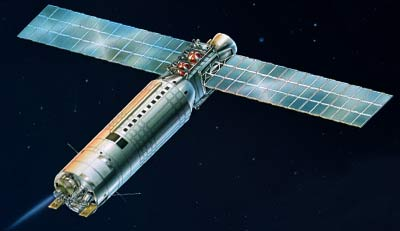
\includegraphics[width = 80mm]{figures/sert-2} & \includegraphics[width = 60mm]{figures/SERT2_Axes} \\
	SERT-2, Source: NASA & SERT-2 Reflectance Model 
	
	\end{tabular}
	\caption{SERT-2 vs Reflectance Model}
	\label{sert_model}
\end{figure}

The geometric model for SERT-2 can be see in figure \ref{sert_model}. The reflectance properties used for each panel were a specular reflectance of 0 and a diffuse reflectance of 0.002. This reflects the properties of matte paint which reflects entirely diffusely. The diffuse coefficient value seems low, although a realistic range of values is not described in the original publication of the Phong model, nor is it described in similar research applying the Phong model \cite{phong_brdf} \cite{SpaceObjectCharacterization} \cite{StateAndParameter} \cite{Kaasalainen_LCI}. This value was empirically estimated to best fit the measured data.

Obviously there is nothing to compare these estimates with as the true angular velocity of SERT-2 is unknown. However, in figure \ref{sert_table} the angular velocity and measurement dates are reported for the successful trials. Since it is assumed that SERT-2 is spinning about a fixed axis, it would be expected that the angular velocity in the ECI frame would all match. This is not the case however.

It is interesting to note that in the body frame, the majority of the solutions show SERT-2 primarily spinning about its Z axis in body frame. This corresponds to it spinning about its length, meaning that the solar panels would be moving rapidly. It would then be expected that some high frequency oscillations would appear in the generated light curve, however none are visible in figure \ref{sert-2_results}. This implies that this solution converged to an attitude in which the contribution of the solar panels was minimized.

% Table generated by Excel2LaTeX from sheet 'datatable'
\begin{table}[H]\label{sert_table}
	\centering
	
	\begin{tabular}{|l|r|r|r|r|r|r|}
		\hline Measurement Date & X Body & Y Body & Z Body & X ECI & Y ECI & Z ECI \\
		\hline 2018-06-02 & -0.03838 & 0.099123 & 0.276464 & -0.03607 & -0.20629 & -0.20946 \\
		\hline 2018-06-15 & 0.094913 & 0.307434 & -0.29946 & 0.4386 & -0.0136 & 0.025415 \\
		\hline 2018-06-23 & -0.0934 & -0.0615 & 0.547375 & 0.448295 & -0.31579 & -0.10693 \\
		\hline 2018-06-27 & 0.004656 & -0.00586 & -0.58329 & 0.29951 & -0.38325 & 0.322009 \\
		\hline 2018-07-02 & 0.012748 & 0.02757 & -0.68151 & -0.08979 & -0.67597 & -0.01929 \\
		\hline 2018-07-07 & 0.107008 & 0.096465 & 0.264944 & 0.206755 & -0.21221 & -0.05632 \\
		\hline 2018-07-16 & -0.00967 & -0.75654 & -0.00129 & -0.53145 & 0.385914 & -0.37562 \\
		\hline 2018-08-10 & -0.06039 & 0.011915 & 0.613305 & -0.33712 & 0.489952 & 0.161957 \\
		\hline 
	\end{tabular}%
	\caption{Final Angular Velocity Vector of SERT-2 According to UKF Estimates.}
\end{table}%


In figure \ref{sert-2_results} the results from one set of data are shown. These are presented in nearly the same manner as the trials in case 1 of the simulated trials. Here the angular velocity is presented in the body frame and the ECI frame (rather than the observation frame). The comparison between the light curve produced by the state estimate and the real data rare shown in addition to their residual. Finally, the MRPs are provided.

In this case the only quantity which can be compared are the measured light curve and the one generated by the state estimate. By looking at the light curve comparison it can be seen that the estimated state was generally able to predict the macroscopic trends of the data. This is a promising result which implies at least some success.

The angular velocities in both the body and ECI frame both converge to fairly constant values which is expected. Additionally the MRPs settled into a stable set of solutions. The strange behavior around 20 seconds in the MRP plot is caused by the UKF updating the MRP estimate very near the threshold of the flip from MRP to shadow parameter causing it to switch back and forth.

\begin{figure}[H]
	\begin{tabular}{cc}
		\includegraphics[width = 50mm]{figures/Sert_Success/BODY} &
		\includegraphics[width=50mm]{figures/Sert_Success/CURVE} \\
		Angular Velocity in Body Frame & Light Curve Comparison \\
		\includegraphics[width = 50mm]{figures/Sert_Success/ECI} &
		\includegraphics[width = 50mm]{figures/Sert_Success/MRP} \\
		Angular Velocity in ECI Frame & Modified Rodrigues Parameter Estimates
	\end{tabular}
	\caption{Convergence of a solution using real data of SERT-2.}
	\label{sert-2_results}
\end{figure}


\subsection{Ajisai (EGS)}

Ajisai was a mission launched on August 13th, 1986 and was primarily intended as a dummy payload for the H-I launch vehicle. \cite{ajisai_jaxa} Ajisai is essentially a sphere covered with 1,436 corner cube reflectors and 318 mirrors. \cite{ajisai} Its secondary mission (after being mass) was to determine the exact position of the more isolated Japanese islands. \cite{ajisai_jaxa}

Because this spacecraft is so old and because it is a sphere, it is highly likely that it is spinning about its major axis and the simpler UKF formulation can be applied once more.

\begin{figure}[!ht]
	\begin{tabular}{cc}
	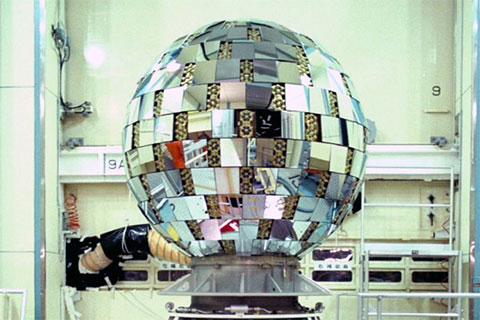
\includegraphics[width = 90mm]{figures/ajisai.jpg} & \includegraphics[width = 60mm]{figures/AJISAI_Axes} \\
	AJISAI, Source: JAXA & AJISAI Reflectance Model
	\end{tabular}
	\caption{AJISAI vs Reflectance Model}
\end{figure}



The geometry of the spacecraft is simply a large set of reflective panels. Being mirrors, these panels will have very high specular reflectance and almost no diffuse reflectance. The corner cube reflectors designed to reflect light back to its source. For this thesis, that source is the sun, and so the corner cube reflectors can be assumed to contribute nothing to the lightcurve. Thankfully, the positions of each corner cube reflector were documented, and the panel locations can be inferred from them.

\begin{figure}
	\centering
	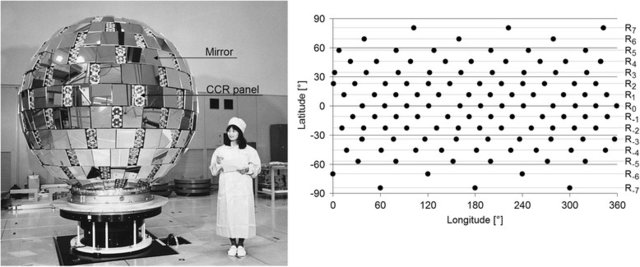
\includegraphics[width = 150mm]{figures/ajisai_panels.jpg}
	\caption{AJISAI with Engineer [Left]. Corner Cube Reflector Locations [Right] \cite{ajisai}}
\end{figure}



The reflective properties used in this spacecrafts model was as specular reflectance of 0.002 and a diffuse reflectance of 0. These values were empirically estimated to best fit the measured data. It can be seen in figure \ref{ajisa_fail} that the measurement model was unable to find an attitude which could recreate the magnitude of the measured data. This was the case for all attempts to filter data collected from this spacecraft.

Had the measurement model agreed with results, it still would have been a challenge for the UKF to converge to an accurate solution as AJISAI is roughly a sphere and its light curve is expected to vary only slightly as a function of attitude. Very high quality data would be needed to capture the detail necessary to discern attitude.

Figure \ref{ajisa_fail} shows a trial with AJISAI data in which a solution was found but which did not fit the data. This is due to the large discrepancy between the true optical properties and the ones assigned to the model. It can be seen that even though a constant angular velocity is reached in the body frame, the light curve generated by this state estimate is significantly off from the real data. Additionally, by looking at the angular velocity in the ECI frame, it can be seen that the UKF had difficulty converging to a set of MRPs. It is likely that the attitude converged upon simply minimized the total brightness.

\begin{figure}[H]
	\begin{tabular}{cc}
		\includegraphics[width = 50mm]{figures/Ajisai_Fail/BODY} &
		\includegraphics[width=50mm]{figures/Ajisai_Fail/CURVE} \\
		Angular Velocity in Body Frame & Light Curve Comparison \\
		\includegraphics[width = 50mm]{figures/Ajisai_Fail/ECI} &
		\includegraphics[width = 50mm]{figures/Ajisai_Fail/MRP} \\
		Angular Velocity in ECI Frame & Modified Rodrigues Parameter Estimates
	\end{tabular}
	\caption{Measurement model mismatch with real data from AJISAI.}
	\label{ajisa_fail}
\end{figure}

\subsection{Second Stage Ariane-40 R/B}

The final object analyzed in this thesis was the second stage of an Ariane-40 rocket. This particular rocket body was launched on September 26th, 1993 \cite{Ariane_Date}. Roughly speaking, the geometry of this debris is roughly cylindrical and be expected to be rotation about its major axis. Therefore the same UKF formulation was applies as the previous two objects. Additionally, being a rocket body, fuel left over is expected to be removing angular momentum through friction which 
increases the likelihood that it is spinning about its major axis.

\begin{figure}[ht]
	\begin{center}
		\includegraphics[width = 60mm]{figures/ARIANE_Axes}
	\end{center}
\caption{Ariane-40 R/B Reflectance Model}
\end{figure}



The reflectance properties used for this model were, once again, a specular reflectance of 0 and a diffuse reflectance of 0.002 . These values were empirically estimated to best fit the measured data.

The UKF managed to converge to a solution in 6 of the 8 trials. Figure \ref{ariane_table} shows the final angular velocities for the Ariane-40 R/B trials. It can be seen that in the body frame the majority of the solutions primarily lie along the Z axis. This is unsurprising as the Z axis of a cylinder has the least effect on the light curve. This means that there should be a large uncertainty about this axis leading to larger values.

Given the results of the simulated results presented in case 1, it was shown that the cylinder geometry had the smallest uncertainty about the Z axis. This is believed to be due to approximating the geometry with a small number of flat surfaces. Therefore the results from the case 1 trials cannot be used to interpret the data. Not only is this low uncertainty about the Z axis an artifact of approximation, the real object being studied is a true cylinder not a series of flat surfaces. The effect of approximating a cylinder with multiple surfaces is unknown. 

Similarly to Sert-2, this object was assumed to be spinning about a fixed axis. It is then expected that any solution generated by the UKF would produce the same angular velocity in ECI with every dataset. As with SERT-2, this was not the case.

% Table generated by Excel2LaTeX from sheet 'datatable'
\begin{table}[htbp]
	\centering
	
	\begin{tabular}{| l | r | r | r | r| r | r |}
		\hline Measurement Date & X Body & Y Body & Z Body & X ECI & Y ECI & Z ECI \\
		\hline 2018-09-2 & -0.00119 & 0.001628 & 0.950441 & 0.093358 & -0.87499 & 0.359184 \\
		\hline 2018-10-09 & 0.011574 & 0.040714 & 0.088763 & 0.095156 & 0.02459 & 0.003341 \\
		\hline 2018-10-20 & 0.008365 & 0.013743 & 0.005531 & -0.01437 & 0.00181 & 0.00893 \\
		\hline 2018-10-23 & 0.001357 & -0.00594 & -0.2812 & -0.24557 & 0.110988 & -0.08052 \\
		\hline 2018-10-26 & -0.01314 & -0.02531 & -0.22751 & -0.14322 & 0.173103 & 0.045802 \\
		\hline 2018-10-29 & 0.009859 & -0.01175 & -0.9638 & 0.264907 & 0.904247 & -0.20324 \\
		\hline 
	\end{tabular}%
	\caption{Final Angular Velocity Vector of Ariane-40 R/B According to UKF Estimates.}
	\label{ariane_table}
\end{table}%

In figure \ref{ariane_results} the results from one set of data are shown. These are presented in nearly the same manner as the trials in case 1 of the simulated trials. Here the angular velocity is presented in the body frame and the ECI frame (rather than the observation frame). The comparison between the light curve produced by the state estimate and the real data rare shown in addition to their residual. Finally, the MRPs are provided.

It can be seen that the UKF does find a solution which minimized the residual, however the data provided for this spacecraft was mostly very flat. This is likely due to the spacecraft spinning so slowly that variations in the data are lost in the noise.

This limits the interpretability of the results, as the signal is so faint that it is unlikely to be sufficient for concrete results. However, the UKF does converge on a solution with near zero angular velocity in the X and Y body axes and only angular velocity in the Z axis. Again, the Z axis in the body frame corresponds to the length of the cylinder and is expected to have a minimal effects of the light curve.
\begin{figure}[!ht]
	\begin{tabular}{cc}
		\includegraphics[width = 50mm]{figures/Ariane_Success/BODY} &
		\includegraphics[width=50mm]{figures/Ariane_Success/CURVE} \\
		Angular Velocity in Body Frame & Light Curve Comparison \\
		\includegraphics[width = 50mm]{figures/Ariane_Success/ECI} &
		\includegraphics[width = 50mm]{figures/Ariane_Success/MRP} \\
		Angular Velocity in ECI Frame & Modified Rodrigues Parameter Estimates
	\end{tabular}
	\caption{Convergence of a solution using real data of Ariane-40 R/B.}
	\label{ariane_results}
\end{figure}


\subsection{Overall Results}

This thesis confirms that is is possible to determine the attitude of a spacecraft using an Unscented Kalman Filter on simulated data. This was possible in cases in which an object is spinning about a fixed axis as well as when an object is tumbling. It was also demonstrated that any attitude solution which fits the data is not unique, and that in some cases a there is a predictable, geometric relationship between some solutions.

Using data collected from SERT-2 and an Ariane-40 Rocket Body the UKF was able to present a plausible solution given the data. However this is unverifiable since the true angular velocity and attitude are unknown. 

Finally, a large discrepancy was noticed between the light model and the measured data in which the model predicted significantly brighter measurements than the collected data in the case of AJISAI. This is potentially due to unmodeled atmospheric effects,  